%*********************************************************************************
% A LaTeX (non-official) template for University of Birmingham
% Copyright (C) 2017 James Li
% Version: 1.0
% Author: James Li <hanlinli.com>
%*********************************************************************************


%***************************   Base   *******************************
\documentclass[a4paper, 12pt]{article}

\usepackage[utf8]{inputenc}
\usepackage{amssymb}
\usepackage{amsmath}
\usepackage{booktabs}
\usepackage{geometry}
\geometry{left=2.5cm,right=2.5cm,top=2.5cm,bottom=2.5cm}
\usepackage{graphicx}
\usepackage{catchfilebetweentags}
\usepackage{float}
\usepackage{caption}
\usepackage{subfigure}
\usepackage{diagbox}
\usepackage{enumitem}
\makeatletter
\newcommand{\rmnum}[1]{\romannumeral #1}
\newcommand{\Rmnum}[1]{\expandafter\@slowromancap\romannumeral #1@}
\makeatother
\newcommand{\tabincell}[2]{\begin{tabular}{@{}#1@{}}#2\end{tabular}}
%***************************    Base   ***************************
\setlength{\parindent}{0pt}          % 取消首行缩进
\setlength{\parskip}{0.8em}          % 设置段落间的空隙（高度约等于一个字符）


\begin{document}
%***************************  Construct  ***************************
\begin{titlepage}
    \begin{center}
    
\includegraphics[width=0.2\textwidth]{Figures/BirminghamUniversityCrest}\\
    \LARGE \textbf{UNIVERSITY OF BIRMINGHAM}\\[1.25cm]

    \LARGE \textbf{Energy-Efficient Visual Control of a Self-Balancing Robot using Spiking Neural Networks: A Neuromorphic Approach at the Edge }\\[0.55cm]

    \large \textbf{by}\\[0.35cm]
    \large \textbf{Han Yang}\\
    \large \textbf{2928212}\\[0.45cm]
    
    \large \textsl{Supervised by} \textbf{Neil Cooke}\\[2.25cm]
	\normalsize \textsl{Dissertation Submitted in Partial Fulfilment of the degree of} \\
    \large \textbf{Electrical and Computer Engineering}\\
    \textbf{20/7/2026}\\[5.25cm]
    \end{center}

\begin{flushright}   

College of Engineering and Physical Sciences\\
The University of Birmingham\\
Edgbaston, Birmingham, UK
\end{flushright}

\end{titlepage}

\pagenumbering{Roman}
\include{Construct/Firstpage}
\newpage

\begin{abstract}
   Visual recognition and control in mobile robotics typically relies on computationally intensive Convolutional Neural Networks(CNNs),
   which poses significant challenges for battery-powered embedded systems, particularly dynamically unstable platforms such as self-balancing 
   robots. Conventional frame-based CNNs process redundant video data regardless of scene dynamics, resulting in substantial energy consumption 
   and processing latency that constrain real-time performance at the edge.

To address these limitations, this dissertation proposes a novel neuromorphic visual control framework based on the Robot Operating System 
(ROS 2 Humble). The system utilizes Difference Encoding to simulate biological retinal mechanisms for dynamic feature extraction and integrates 
a custom-designed Spiking Convolutional Neural Network (SCNN). Furthermore, to bridge the gap between algorithmic complexity and embedded constraints, 
a high-performance C++ inference engine is developed to deploy the SNN within the real-time control loop of the robot.

Experimental results demonstrate that in visual line-following and target tracking tasks, the proposed SNN architecture maintains control accuracy 
comparable to traditional deep learning approaches while reducing theoretical Synaptic Operations (SOPs) by approximately [X]
% compared to isomorphic CNNs. These findings validate the potential of Spiking Neural Networks for enabling energy-efficient, low-latency visual control in edge robotics.
\end{abstract}
\clearpage
\newpage
\input{Construct/Contents}
%***************************  Construct  ***************************




\clearpage
\pagenumbering{arabic}
%***************************  Sections   ***************************
\section{Introduction}

\subsection{Background and Motivation}
The proliferation of autonomous mobile systems has revolutionized sectors
ranging from industrial logistics to domestic services. At the core of these 
systems lies visual perception and control, which enables robots to perceive and 
interpret unstructured environments and execute complex navigation tasks[1]. In recent
years, Convolutional Neural Networks(CNNs) have established themselves as the state-of-art solution
for robotic vision due to their superior performance in feature extraction 
and pattern recognition[2].\\

However, the deployment of Deep Learning models on some mobile robotic platforms
(most of them are resource-constrained) introduces a fundamental trade-off between 
computational performance and energy efficiency. Unlike cloud-based AI systems with
almost unlimited computational and energy resources, mobile robots and 
embedded systems-- especially micro-robots and self-balancing robots-- 
operate under significant constraints and challenges due to their limites computational resources,
including memory, processing power, and energy consumption[3].

The continuous processing of 
computionally intensive CNNs on battery-powered embedded processors often leads to
rapid depletion and thermal throttling, which severely limites the operational duration
of the robot and its ability to perform real-time tasks.\\

To address these challenges, Neuromorphic Computing has emerged as a promising paradigm
shift in embedded Artificial Intelligence. Inspired by the energy-efficient mechanisms
of the biological brain, Spiking Neural Networks(SNNs) process information using discrete,
sparse events(Spikes) rather than continuous numerical values, can offer
order-of-magnitude improments in energy efficiency compared to traditional Artificial Neural
Networks(ANNs)[5]. Consequently, investigating the application of SNNs in Edge Robotics
represents a critical frontier in modern robotic engineering.

\subsection{Problem Statement}
Despite their theoretical potential, the pratical deployment of SNNs on 
physical rototic platforms faces several critical engineering challenges:
\begin{description}
    \item[Computational Efficiency on Non-Neuromorphic Hardware:] While SNNs are 
    designed for specialized neuromorphic 
    chips (e.g., Intel Loihi), most edge robots, such as the Yahboom self-balancing 
    platform,
     rely on general-purpose microcontrollers like the STM32 and ESP32.
      Achieving high-performance SNN inference on these platforms requires rigorous 
      optimization of software-hardware co-design.
    
    \item[Sensory Integration and Real-time Control:] Autonomous systems such as two-wheeled
    self-balancing robots are dynamically unstable and require millisecond-level feedback loops. 
    Conventional frame-based vision sensors generate redundant data, which contradicts 
    the event-driven nature of SNNs. Developing a visual encoding mechanism that can bridge 
    frame-based input with spike-based processing isessential for maintaining system stability.

    
    \item[The Sim-to-Real Gap:] Many SNN studies remain confined to theoretical simulations
    or static dataset benchmarks. There is a pressing need for empirical research that demonstrates
    the feasibility of SNNs in managing closed-loop, real-time control tasks on physical hardware.
\end{description}

\subsection{Research Aims and Objectives}
The primary aim of this research is to design and implement a high-performance,
energy-efficient visual control framework for a self-balancing robot, leveraging the sparse compurting
characteristics of SNNs. The research will focus on achieving real-time, colsed-loop
navigation by optimizing the synergy between neuromorphic algorithms and embedded hardware.
To achieve this aim, the following objectives have been established:
\begin{enumerate}[label=\textbf{Objective \arabic*:}, leftmargin=*]
    \item \textbf{Development of a Hierarchical Control Architecture}\newline
    To establish a multi-layer control system using ROS 2 Humble. This involves
    utilizing an ESP32-S3 as a high-speed communication gateway to bridge the high-level
    SNN cognitive logic(running on a host machine) with the low-level reflexive control
    (implemented on an STM32F103). The architecture will leverage micro-ROS to ensure 
    synchronized data exchange between the SNN decision-making and the PID balancing loops.
    
    
    \item \textbf{Design of a Retina-inspired Visual Encoder}\newline
    To develop a visual encoding scheme based on temporal difference algorithms. 
    By computing the pixel-level intensity changes between successive frames,
    the system converts standaed RGB video streams into sparse, event-based spike
    tensors. This process aims to minimize redundant computation at the edge, mirroring
    the biological efficiency of the human retina.
    
    \item \textbf{Implementation of an Optimized C++ Inference Engine}\newline
    To engineer a dedicated SNN inference engine using the Eigen library within a C++
    environment. Utilizing software-hardware co-design techniques, this objective 
    focuses on minimizing processing latency to meet the millisecond-level responsiveness
    required for dynamically unstable platforms.

    \item \textbf{Performance Evalution and Benchmarking}\newline
    To quantitatively access the navigation accuracy and energy efficiency of the system.
    Using Synaptic Operations(SPOs) as the primary metric, the SNN-based controller will
    be benchmarked against traditional CNNs to validate its energy-saving potential
    in edge robotics applications.
\end{enumerate}

\subsection{Research Significance}
This research contributes to the field of Edge Artifical Intelligence(Edge AI) by
bridging the gap between biological inspiration and practical robotic engineering:

\begin{enumerate}[label=\textbf{\arabic*.}, leftmargin=*]
    \item \textbf{Practical Framework for Spike-based Robotics} \newline
    By implementing SNNs on a cost-effective, multi-processor platform(integrating STM32
    and ESP32), this work provides a scalable bileprint for the transition from theoretical
    simulation to physical deployment. It validates the robustness of event-driven vision
    in stabilizing dynamically unstable systems, offering a viable path for the development
    of long-endurance autonomous embedded devices.
    
    \item \textbf{Advancement of Software-Hardware Co-optimization} \newline
    The research demonstrates a rigorous co-optimization straegy, where the high-level C++
    SNN engine is harmomized with the low-level micro-ROS communicationlayer. 
    This approach addresses the critical constraints of Edge Intelligence,
     such as limited memory and power budgets, 
     while ensuring the millisecond-level responsiveness required for real-time control.
    
    \item \textbf{Integration of Neuromorphic Theory and Nanostructure Horizons}\newline 
    This dissertation establishes a computational foundation for the future migration of AI 
    from general-purpose CPUs to specialized neuromorphic architectures. By validating SNN 
    algorithmic efficiency on standard CMOS-based hardware, the research provides critical 
    performance benchmarks and architectural insights. These findings are essential for the 
    future design of dedicated Neuromorphic Systems-on-Chip (NSoC), facilitating the evolution 
    toward more bio-plausible and energy-efficient digital integrated circuits.
\end{enumerate}

\subsection{Thesis Structure}
The remainder of this dissertation is organized into the following seven chapters:

\begin{itemize}[leftmargin=*]

    \item \textbf{Chapter 2: Literature Review} examines the theoretical foundations of 
    Spiking Neural Networks (SNNs) alongside classical control theories. It reviews the 
    state-of-the-art in neuromorphic sensing, Real-Time Operating Systems (RTOS) for 
    robotics, and the stability challenges inherent in inverted pendulum systems.

    \item \textbf{Chapter 3: System Methodology} proposes a decoupled hierarchical architecture. 
    It details the mathematical modeling of the self-balancing robot, the design of the cascaded 
    PID control loops, and the development of a ``Retina-inspired'' visual encoding algorithm for 
    spike-based perception.

    \item \textbf{Chapter 4: Implementation and Engineering} describes the multi-processor hardware
     integration involving the STM32F103 and ESP32-S3. This chapter focuses on the embedded software 
     engineering aspects, including RTOS task prioritization, micro-ROS middleware configuration, and 
     the development of an optimized C++ SNN inference engine.

    \item \textbf{Chapter 5: Experiments and Results} presents empirical data from physical robot trials.
     It evaluates the system's performance across multiple dimensions, including balancing stability (pitch jitter),
      navigation accuracy, and computational energy efficiency quantified by Synaptic Operations (SOPs).

    \item \textbf{Chapter 6: Discussion} provides a critical analysis of the experimental findings, 
    focusing on the trade-offs between biological plausibility and real-time engineering constraints. 
    It also discusses the system's robustness in Edge AI scenarios.

    \item \textbf{Chapter 7: Conclusion} summarizes the key engineering contributions and academic insights
     of the research, offering recommendations for future advancements in neuromorphic embedded systems and 
     hardware-in-the-loop control.

\end{itemize}

\ExecuteMetaData[table]{parameters}

\newpage
\section{Literature Review}



\subsection{Neuromorphic Computing and Spiking Neural Networks}

\subsubsection{From Frame-based to Event-based Perception}

Conventional Artificial Neural Networks (ANNs), particularly Convolutional Neural Networks (CNNs), 
rely on dense, frame-synchronous processing, where information is represented by continuous-valued 
floating-point activations across all neurons regardless of input characteristics. While effective 
for static image recognition tasks, this paradigm exhibits inherent computational redundancy: 
the entire pixel array is re-evaluated via matrix multiplications at each time step, regardless 
of temporal variations in the scene. 

For a dynamically unstable system such as a self-balancing robot—which can be modeled as an inverted 
pendulum subject to perturbations—this redundancy imposes critical penalties:
\begin{itemize}
    \item A fixed latency floor bounded by the framerate (e.g., 33 ms at 30 Hz, 16.7 ms at 60 Hz),
    \item Excessive computational overhead with every frame, even when the visual scene remains static,
    \item Bandwidth saturation of communication channels between vision processing and control modules,
    \item Potential destabilization of high-frequency feedback loops that demand responsiveness in the 
    millisecond range.
\end{itemize}

From a power perspective, each Multiply-Accumulate (MAC) operation—the fundamental building block 
of neural computation—consumes substantial energy on traditional CPUs and GPUs. A typical modern 
CPU requires 1-10 picojoules per MAC operation, depending on clock speed and circuit technology. 
For high-resolution visual inputs (e.g., 320×240 pixels, 3 channels) processed through a CNN with 
multiple convolutional layers, the total energy expenditure per inference can reach hundreds of 
millijoules, which is prohibitive for battery-powered systems \cite{gallego2020event}.


\begin{figure}[htbp]
    \centering
    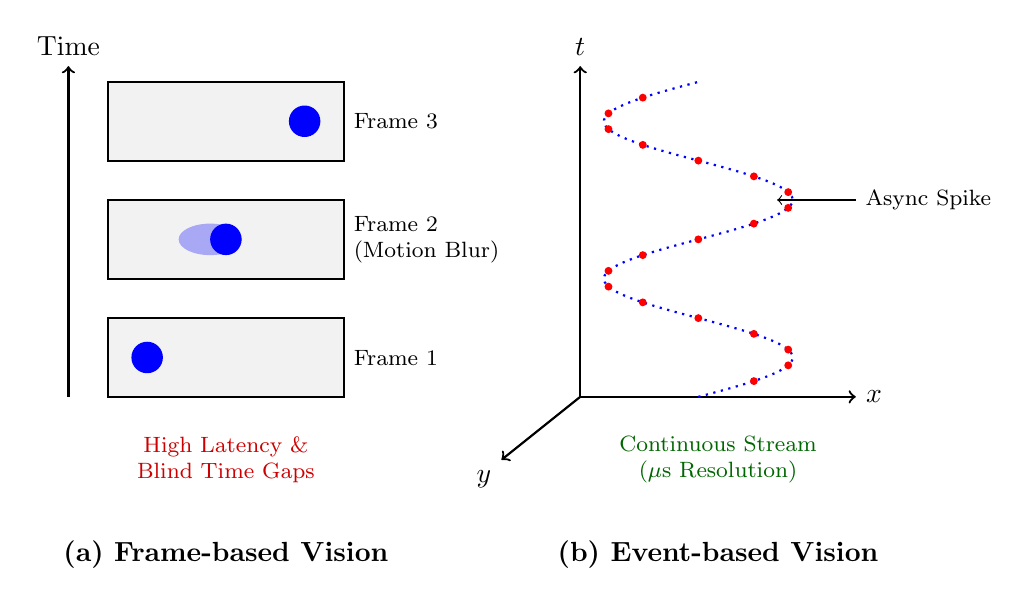
\begin{tikzpicture}
        % ================= 左图：Frame-based =================
        \begin{scope}[shift={(-3.5,0)}]
            % 1. 画时间轴箭头
            \draw[->, thick] (-0.5, 0) -- (-0.5, 4.2) node[above] {Time};
            
            % 2. Frame 1 (t=0)
            \draw[thick, fill=gray!10] (0, 0) rectangle (3, 1);
            \fill[blue] (0.5, 0.5) circle (0.2); 
            \node[right, font=\footnotesize] at (3, 0.5) {Frame 1};
            
            % 3. Frame 2 (t=1) - 模拟运动模糊
            \draw[thick, fill=gray!10] (0, 1.5) rectangle (3, 2.5);
            \fill[blue, opacity=0.3] (1.3, 2.0) ellipse (0.4 and 0.2); 
            \fill[blue] (1.5, 2.0) circle (0.2); 
            \node[right, font=\footnotesize, align=left] at (3, 2.0) {Frame 2\\(Motion Blur)};
            
            % 4. Frame 3 (t=2)
            \draw[thick, fill=gray!10] (0, 3.0) rectangle (3, 4.0);
            \fill[blue] (2.5, 3.5) circle (0.2); 
            \node[right, font=\footnotesize] at (3, 3.5) {Frame 3};
            
            % 5. 缺点描述 (红色文字)
            \node[red!80!black, font=\footnotesize, align=center] at (1.5, -0.8) {High Latency \&\\Blind Time Gaps};

            % 6. 【修改位置】标题移动到底部
            \node[font=\bfseries] at (1.5, -2.0) {(a) Frame-based Vision};
        \end{scope}

        % ================= 右图：Event-based =================
        \begin{scope}[shift={(2.5,0)}]
            % 1. 画 3D 坐标轴 (x, y, t)
            \draw[->, thick] (0,0) -- (3.5,0) node[right] {$x$};
            \draw[->, thick] (0,0) -- (0,4.2) node[above] {$t$};
            \draw[->, thick] (0,0) -- (-1,-0.8) node[below left] {$y$};
            
            % 2. 画螺旋轨迹 (Spikes)
            \draw[blue, thick, dotted] plot[domain=0:4, samples=100] ({1.5 + 1.2*sin(180*\x)}, \x);
            
            % 3. 添加脉冲点 (Spikes)
            \foreach \t in {0.2, 0.4, ..., 3.8} {
                \fill[red] ({1.5 + 1.2*sin(180*\t)}, \t) circle (0.05);
            }
            
            % 4. 优势描述 (绿色文字)
            \node[green!40!black, font=\footnotesize, align=center] at (1.75, -0.8) {Continuous Stream\\($\mu$s Resolution)};
            
            % 5. 标注 Spike Event
            \draw[<-, thin] (2.5, 2.5) -- (3.5, 2.5) node[right, font=\footnotesize] {Async Spike};

            % 6. 【修改位置】标题移动到底部
            \node[font=\bfseries] at (1.75, -2.0) {(b) Event-based Vision};
        \end{scope}

    \end{tikzpicture}
    
    \caption{Visual comparison of acquisition paradigms. \textbf{(a)} Standard frame-based 
    cameras capture discrete snapshots with fixed intervals, suffering from blind spots between
     frames and motion blur. \textbf{(b)} Event-based sensors 
     record asynchronous spikes with microsecond resolution, forming a continuous trajectory in 
     space-time ideal for high-speed control.}
    \label{fig:frame_vs_event}
\end{figure}


In contrast, Spiking Neural Networks (SNNs)—conceptualized as the \emph{third generation} of neural 
networks—introduce a fundamental paradigm shift towards neuromorphic, event-driven computing inspired 
by biological neural systems. Rather than encoding information in continuous activation values, SNNs 
represent information in the precise timing and frequency of discrete, binary impulses known as ``spikes.'' 
This asynchronous processing mechanism confers multiple critical advantages for embedded robotic control:

\begin{enumerate}
    
\item \textbf{Temporal Sparsity and Energy Efficiency:}
Unlike ANNs where every neuron produces an output at every timestep, in SNNs neuronal activation is 
\emph{conditional and event-driven}. A neuron fires (emits a spike) only when its membrane potential 
accumulates sufficient synaptic inputs to breach a firing threshold. Mathematically, the membrane 
potential dynamics can be described by the Leaky Integrate-and-Fire (LIF) model:

$$V_i(t) = \tau \frac{dV_i}{dt} + V_i = \sum_j w_{ij} \sum_f \delta(t - t_f^j) + I_{\text{ext}}$$

where $V_i(t)$ is the membrane potential, $\tau$ is the time constant, $w_{ij}$ is the synaptic weight, 
$t_f^j$ are spike times from pre-synaptic neuron $j$, and $I_{\text{ext}}$ is external input. A spike 
is generated when $V_i > V_{\text{threshold}}$.

Consequently, static background elements (e.g., unmoving walls, floors in a fixed environment) in a 
visual navigation task elicit negligible spiking activity, resulting in extremely high sparsity (often 
>95\% of potential operations are skipped). This sparsity allows the hardware to replace the power-hungry 
Multiply-Accumulate (MAC) operations typical of conventional ANNs with energy-efficient, event-driven 
Accumulate (AC) operations that require no multiplication when a neuron does not spike \cite{roy2019towards}. 
This effectively decouples computational cost from input resolution—a key advantage for high-resolution 
vision systems. Research has demonstrated that SNNs can achieve order-of-magnitude reductions (10-100×) 
in energy consumption compared to isomorphic CNNs, making them particularly attractive for battery-constrained 
platforms with operational lifetimes measured in hours rather than minutes \cite{pham2019spiking}.


\item \textbf{High Temporal Resolution and Low Latency:} 
Unlike frame-based systems constrained by the Nyquist sampling rate of standard cameras (e.g., a fixed 
33 ms latency at 30 Hz), SNNs operate on continuous time dynamics with sub-millisecond temporal precision. 
The membrane potential evolves continuously, and spikes can be generated at any time within the simulation 
timestep (typically 1 ms or finer). This allows for pseudo-continuous processing of visual inputs, theoretically 
enabling microsecond-level responsiveness to sudden environmental changes.

For self-balancing robots, this property is imperative. The system operates with poles at the origin in the 
complex plane (marginally stable or unstable depending on physical parameters), meaning any disturbance grows 
exponentially. With a typical control period of 10-20 ms, introducing latency can significantly degrade closed-loop 
stability or increase control effort. SNNs' inherent low latency (often <5 ms total for inference) enables tighter, 
more responsive feedback loops compared to frame-based approaches that inherently incur one frame period of delay.

\end{enumerate}

Biologically, this event-driven mechanism mirrors the operation of biological neurons in the brain. Cortical 
neurons fire sparsely (at rates of 0.1-10 Hz on average), yet encode rich temporal and spatial information 
through precise spike timing. The brain's energy consumption—approximately 20 watts for the human brain with 
86 billion neurons—translates to mere microjoules per neuron per second, a remarkable efficiency that ANNs 
with their continuous activation paradigm cannot match \cite{lennie2003cost}.





\subsubsection{Neuronal Models and Spike Generation Mechanisms}

Several spiking neuron models have been proposed in the literature, each trading off biological 
fidelity against computational complexity. The Leaky Integrate-and-Fire (LIF) model, described above, 
is widely adopted for its simplicity and computational efficiency. However, alternative models such as 
the Hodgkin-Huxley model, Izhikevich model, and Exponential Integrate-and-Fire (ExIF) model offer 
varying levels of detail:

\begin{description}
    \item[Hodgkin-Huxley Model:] Captures voltage-gated ion channel dynamics with four state variables 
    (membrane potential and three gating variables). Biologically accurate but computationally expensive 
    ($\mathcal{O}(10)$ operations per neuron per timestep).
    
    \item[Izhikevich Model:] A two-variable reduced model that exhibits diverse firing patterns (tonic spiking, 
    bursting, etc.) while remaining relatively efficient ($\mathcal{O}(4)$ operations per neuron per timestep).
    
    \item[Leaky Integrate-and-Fire (LIF):] The standard in neuromorphic computing, using a single state variable 
    (membrane potential) and a reset mechanism. Highly efficient ($\mathcal{O}(2)$ operations per neuron per timestep).
\end{description}

For embedded deployment on resource-constrained hardware, the LIF model is preferred due to its minimal computational 
footprint and proven effectiveness in pattern recognition tasks. After firing, the neuron's membrane potential is 
typically reset to a resting value $V_{\text{reset}} < V_{\text{threshold}}$, and a relative refractory period is 
often modeled to prevent unrealistically high firing rates.

The output of an SNN layer at timestep $t$ can be expressed as:

$$O_i(t) = \begin{cases} 1 & \text{if } V_i(t) \geq V_{\text{threshold}} \\ 0 & \text{otherwise} \end{cases}$$

This binary output propagates through synaptic connections to post-synaptic neurons, accumulating over multiple 
timesteps to build a temporal encoding of the input signal.


\subsection{Challenges in Deploying SNNs on Embedded Robotics Platforms}

The practical deployment of SNNs on embedded robotic platforms encounters
several critical technical and architectural challenges:

\subsubsection{Conversion and Inference Optimization}

While SNNs offer inherent energy advantages, training them from scratch remains computationally intensive 
due to the non-differentiable nature of the spike function. The discontinuous Heaviside function creates a 
zero gradient almost everywhere, violating the chain rule necessary for standard backpropagation. Several 
workarounds have been proposed:

\begin{enumerate}
    \item \textbf{Surrogate Gradient Methods:} Replace the spike function with a smooth approximation during 
    backpropagation (e.g., sigmoid or tanh) while maintaining the binary spike function during forward pass. 
    This enables direct training but introduces a bias-variance trade-off.
    
    \item \textbf{Spike-Timing-Dependent Plasticity (STDP):} Biologically-inspired learning rules that 
    strengthen synapses when pre- and post-synaptic spikes arrive with specific timing relationships. 
    Computationally efficient but convergence to optimal solutions is not guaranteed.
    
    \item \textbf{ANN-to-SNN Conversion:} Train a conventional ANN with ReLU activations, then map the 
    learned weights to an SNN by calibrating the firing thresholds and simulation time steps. This approach 
    avoids direct SNN training complexity.
\end{enumerate}

The ANN-to-SNN conversion approach has become dominant in recent years, particularly for embedded applications. 
The mapping exploits the similarity between ReLU activations in ANNs and spike counts in SNNs: a ReLU neuron 
outputs its input if positive, zero otherwise. Over multiple timesteps $T$, an SNN neuron can approximate the 
ReLU activation if the total spike count is appropriately scaled:

$$y_{\text{ANN}} = \max(0, x) \approx \frac{1}{T} \sum_{t=0}^{T-1} \text{spike}_i(t)$$

However, this conversion introduces several error sources:

\begin{itemize}
    \item \textbf{Discretization Error:} Converting continuous ReLU outputs to discrete spike counts introduces quantization noise, 
    particularly for small positive activations where rounding errors are significant.
    
    \item \textbf{Temporal Integration Error:} The approximation improves with larger $T$ but increases latency. 
    For closed-loop control, $T$ must be constrained to 10-100 timesteps, limiting the accuracy of representation.
    
    \item \textbf{Threshold Calibration:} The firing threshold must be carefully tuned to balance the spike count 
    distribution across layers. Suboptimal thresholds lead to either excessive sparsity (dead neurons) or high firing 
    rates (loss of energy efficiency).
\end{itemize}

Recent research \cite{rueckauer2017conversion, diehl2015fast} has proposed automated threshold calibration 
algorithms, such as moving threshold or uniform threshold schemes, achieving conversion errors below 5\% on 
standard benchmarks (MNIST, CIFAR-10).

Beyond conversion accuracy, deploying SNN inference on general-purpose microcontrollers (such as STM32F103 or ESP32) 
requires careful optimization of the computation pattern. The event-driven nature of SNNs—where computation is 
proportional to the number of spikes rather than the total number of synapses—contradicts the vectorized, 
matrix-based acceleration available on conventional CPUs. Most CPU architectures are optimized for dense matrix 
operations (via SIMD/NEON instructions), not sparse, irregular computations. This creates a critical gap:

\begin{itemize}
    \item \textbf{FLOPS Utilization:} A dense CNN achieves >80\% of peak FLOPS on modern hardware. An SNN with 95\% 
    sparsity achieves only ~5\% utilization, since most MACs are skipped and the CPU pipeline remains idle.
    
    \item \textbf{Memory Bandwidth:} SNNs require pointer chasing and index calculations to locate non-zero weights, 
    generating cache misses and memory stalls that can degrade performance despite computation being sparse.
    
    \item \textbf{Software Overhead:} The event-driven execution model requires bookkeeping (tracking active neurons, 
    managing spike lists) that, while negligible on neuromorphic hardware, can consume significant cycles on CPUs.
\end{itemize}

Specialized inference engines, such as Brian2, NEST, and Nengo, have been developed to mitigate these issues through 
loop fusion, cache-aware data layout, and batch spike processing. However, these frameworks typically target larger 
compute platforms (Linux with >1GB RAM). For embedded microcontrollers with <512KB RAM, custom, hand-optimized C++ 
kernels leveraging Eigen for small matrix operations have proven more practical \cite{pehle2022neuromorphic}.

\subsubsection{Vision-to-Spike Encoding for Frame-based Sensors}

Biological SNNs in sensory cortices interface with specialized neuromorphic sensors (e.g., photoreceptors in the retina, 
mechanoreceptors in the skin) that naturally output spike trains. However, most mobile robotic platforms employ conventional 
frame-based RGB or grayscale cameras for practical and economic reasons: frame-based cameras are mass-produced commodity 
devices with mature manufacturing ecosystems, while neuromorphic event-based cameras (Dynamic Vision Sensors, DVS) remain 
specialized research instruments with limited availability and higher costs ($500-2000 vs. $10-50 for frame-based cameras).

Converting frame-based visual data into sparse spike representations requires an encoding mechanism that bridges the 
temporal sampling paradigm (frames at discrete intervals) with the continuous spike generation of SNNs. Several encoding 
strategies have been proposed in the literature:

\begin{enumerate}
    
\item \textbf{Poisson Encoding:} Each pixel intensity is mapped to a firing probability, and spikes are generated stochastically 
according to a Poisson process with rate proportional to pixel value:

$$P(\text{spike at pixel } i) = \frac{I_i(t)}{I_{\max}}$$

where $I_i(t)$ is the intensity at pixel $i$ and $I_{\max}$ is the maximum pixel intensity (255 for 8-bit images). 
\textbf{Advantages:} Simple to implement, biologically plausible. \textbf{Disadvantages:} Introduces randomness, requires 
many timesteps to converge to accurate rate representation (high latency), and degrades control performance due to stochastic 
jitter in critical feedback signals.

    
\item \textbf{Temporal Difference Encoding:} Compute pixel-level intensity changes between successive frames:

$$\Delta I_i(t) = I_i(t) - I_i(t-1)$$

Spikes are generated when the magnitude of change exceeds a threshold:

$$\text{spike}_i(t) = \begin{cases} 1 & \text{if } |\Delta I_i(t)| > \theta \\ 0 & \text{otherwise} \end{cases}$$

\textbf{Advantages:} Low latency (immediate response to changes), biologically plausible (mimics retinal on-center/off-center 
receptive fields), naturally sparse (static regions produce no spikes). \textbf{Disadvantages:} Sensitive to camera noise 
and illumination changes; threshold selection is critical and may require per-scene calibration. This approach is particularly 
well-suited for self-balancing robots where temporal changes (robot tilt, body motion) are the informative signal, and static 
background regions should indeed produce minimal computation.

    
\item \textbf{Population Coding:} Represent each pixel intensity using multiple neurons with overlapping receptive fields:

$$\text{spike}_{i,j}(t) = \begin{cases} 1 & \text{if } \mu_j - \sigma_j < I_i(t) < \mu_j + \sigma_j \\ 0 & \text{otherwise} \end{cases}$$

where $\mu_j$ and $\sigma_j$ define the tuning of neuron $j$. \textbf{Advantages:} Robust to noise, provides redundancy. 
\textbf{Disadvantages:} Multiplies the number of neurons (and computation) by the population size, increasing latency and 
energy consumption.

\end{enumerate}

For embedded robotic control, temporal difference encoding emerges as the optimal choice, balancing latency requirements 
with sparsity benefits. The threshold $\theta$ can be adapted based on scene statistics (e.g., auto-tuned to generate 
10-30\% sparsity) or learned during system calibration.

The computational cost of encoding is typically negligible compared to neural inference. For a $W \times H \times C$ 
resolution image with $C$ color channels, temporal difference encoding requires $W \times H \times C$ subtraction operations 
and comparisons per frame, totaling $\mathcal{O}(W \times H \times C)$ operations. For 320×240 RGB images, this is only 
230,400 simple operations—orders of magnitude cheaper than CNN inference which may involve millions of MACs.

A critical practical challenge is ensuring temporal synchronization: the visual encoding must operate synchronously with 
the SNN simulation timesteps. If visual frames arrive asynchronously (common with USB cameras), additional buffering and 
interpolation logic may be required, introducing latency and potential desynchronization artifacts.

\subsubsection{Real-time Control Loop Integration}

Self-balancing robots (e.g., Yahboom, DJI Robomaster, custom two-wheeled platforms) operate as dynamically 
unstable mechanical systems, mathematically modeled as an inverted pendulum. The linearized dynamics near 
the balance point are characterized by poles on the imaginary axis (marginally stable) or in the right 
half-plane (unstable), depending on friction and other parasitic effects:

$$\ddot{\theta} = \frac{mg\ell}{I} \theta + \frac{C_f}{I} \dot{\theta} + \frac{\tau}{I}$$

where $\theta$ is tilt angle, $m$ is mass, $\ell$ is distance to center of mass, $I$ is moment of inertia, 
$C_f$ is friction damping, and $\tau$ is motor torque input. For a typical self-balancing robot, the 
unstable pole magnitude ranges from 2-5 rad/s, meaning disturbances grow exponentially with a time constant 
of 200-500 milliseconds. Without active control, the robot tips over within seconds.

Maintaining balance requires a feedback control loop operating at a sufficient frequency. Standard practice 
is to maintain control rates between 50-200 Hz (period: 20-5 ms). This tight real-time requirement creates 
several critical constraints when integrating visual perception:

\begin{enumerate}
    
\item \textbf{Latency Budget:} The total latency from image capture to motor command must not exceed the control 
period. For a 100 Hz control loop (10 ms period), if $t_{\text{capture}} \approx 5$ ms (one frame period), 
$t_{\text{encode}} \approx 1$ ms, and $t_{\text{PID}} \approx 1$ ms, the budget for visual inference is at most 
3-4 ms. Exceeding this budget introduces phase lag in the feedback loop, degrading stability margins.

Delay in a feedback system reduces phase margin. For a system with open-loop transfer function $G(s)H(s)e^{-sL}$ 
(where $L$ is latency), the closed-loop phase margin decreases by approximately $\omega_c \cdot L$ radians (where 
$\omega_c$ is cross-over frequency). For a 100 Hz control loop with $\omega_c \approx 10$ rad/s, a 10 ms latency 
introduces 100 milliradians $\approx 5.7°$ phase loss, which can erode the phase margin from a comfortable 60° to 
a risky 30°, potentially triggering instability under disturbances.

    
\item \textbf{Deterministic Timing:} While latency is important, variability (jitter) is equally critical. Control 
theory dictates that jitter in the feedback loop can excite resonances and destabilize an otherwise stable system. 
SNNs inherently exhibit variable latency due to:
    \begin{itemize}
        \item Stochastic spike generation (if using Poisson encoding, latency varies randomly),
        \item Data-dependent computation (denser regions produce more spikes, longer computation),
        \item Memory access patterns (cache misses on microcontrollers cause unpredictable delays).
    \end{itemize}
    
For embedded systems, adhering to hard real-time constraints requires OS-level support (e.g., FreeRTOS with 
priority scheduling) and careful profiling to identify worst-case execution time (WCET). SNNs operating with 
>10\% sparsity can have WCET exceeding their typical latency by 2-3×, necessitating conservative timing analysis.

    
\item \textbf{Feedback Stability Under Delays:} Classical control theory provides tools to analyze stability 
with delay. Using frequency-domain methods (e.g., Nyquist criterion with delay compensation), the critical delay 
threshold $L_{\text{crit}}$ beyond which closed-loop stability is lost can be computed. For typical self-balancing 
robot parameters ($K_p = 50$ for proportional gain, $\omega_n = 5$ rad/s natural frequency), $L_{\text{crit}}$ 
ranges from 40-80 ms. With a 10 ms control latency budget, substantial safety margin remains, but further increases 
would be detrimental.

\end{enumerate}

Additionally, the stochastic nature of SNNs—particularly when trained via surrogate gradient methods or using 
probabilistic encoding—introduces output variability. Unlike deterministic CNNs where the same input always produces 
identical outputs, SNNs may output different spike patterns for identical inputs (if dropout or noisy encoding is 
employed). This output variability, if not carefully managed, can manifest as jitter in control commands and 
potentially destabilize the system \cite{tan2021neuromorphic}.

Integration of SNN inference into the control loop typically follows one of two architectures:

\begin{description}
    \item[Sequential Architecture:] Image capture → Encode → SNN inference → PID control → Motor output, all 
    within one control cycle. Requires sub-millisecond inference to meet latency budgets; feasible only for 
    very small SNNs (few layers, <1000 neurons).
    
    \item[Pipelined Architecture:] Inference and control operate in parallel threads/processes with inter-process 
    communication (IPC). Vision thread processes frame $n$ while control thread executes feedback loop on frame 
    $n-1$. Increases effective throughput but introduces multi-frame latency (20-50 ms), acceptable only for 
    non-critical tasks (navigation planning, obstacle avoidance) not for direct balance stabilization.
\end{description}

For self-balancing robots, the sequential architecture is typically required for stabilization feedback, while 
pipelined operation suffices for higher-level navigation tasks in a hierarchical control system.


\subsection{Large Language Models and Foundation Models in Robotics}

\subsubsection{Overview of Transformer-based Foundation Models}

The emergence of large language models (LLMs)—such as GPT-3 (175B parameters), GPT-4 (estimated 1T+ parameters), 
and open-source alternatives like LLaMA (7B-65B), Mistral (7B), and Qwen (1.8B-72B)—has revolutionized natural 
language understanding and reasoning. These models, trained on massive internet-scale corpora (100GB-10TB of text), 
develop remarkably general capabilities in:

\begin{itemize}
    \item \textbf{Semantic Understanding:} Parsing unstructured natural language into rich semantic representations,
    \item \textbf{Knowledge Integration:} Reasoning over memorized facts and learned patterns from pretraining,
    \item \textbf{Task Adaptation:} Few-shot learning from in-context examples, without explicit parameter updates,
    \item \textbf{Compositionality:} Decomposing complex tasks into subtasks and combining solutions.
\end{itemize}

The extension of LLMs to multimodal settings—particularly vision-language models (VLMs) such as CLIP, Flamingo, 
GPT-4V, and LLaVA (Large Language and Vision Assistant)—enables these semantic capabilities to operate over visual 
inputs. Modern VLMs achieve state-of-the-art performance on visual understanding tasks: visual question answering (VQA) 
with >85\% accuracy, visual reasoning outperforming specialized models, and open-ended description generation with 
human-level quality \cite{openai2023gpt4, alayrac2022flamingo}.

\subsubsection{Vision-Language Models for Robotic Understanding}

In the context of robotic control and navigation, VLMs provide multiple novel capabilities beyond traditional 
computer vision pipelines:

Recent advances in large language models (LLMs) and vision-language models (VLMs) have
demonstrated remarkable capabilities in semantic understanding, reasoning, and knowledge
integration across diverse domains \cite{openai2023gpt4, alayrac2022flamingo}. These foundation models
can be leveraged for high-level robotic task planning and scene interpretation.



\begin{enumerate}
    
\item \textbf{Semantic Scene Understanding and Grounding:} VLMs can process visual inputs to generate rich symbolic 
descriptions of the environment, enabling the robot to reason about high-level scenarios beyond low-level pixel 
features. For example, given a camera frame, a VLM can generate descriptions such as:
    \begin{itemize}
        \item ``A black horizontal line on a white surface, indicating the path to follow,''
        \item ``Obstacles detected: wooden blocks on the right, open space on the left,''
        \item ``Surface type: textured carpet; traction is likely reduced.''
    \end{itemize}

These semantic grounding outputs can guide adaptive behavior: if the VLM detects reduced traction, the robot can 
adjust motor gains or increase control bandwidth. This is substantially richer information than traditional CV 
pipelines (e.g., Hough transforms for line detection) which output only geometric primitives.

    
\item \textbf{Task-level Planning and Instruction Following:} LLMs excel at parsing natural language task descriptions 
and decomposing them into executable steps. A user can instruct the robot in natural language—``Navigate to the marker 
cone and stop in front of it''—and the LLM can decompose this into:
    \begin{enumerate}
        \item Subtask 1: Locate the marker cone in the visual frame (delegate to VLM for visual grounding),
        \item Subtask 2: Compute relative position and bearing to the target,
        \item Subtask 3: Generate motion commands to approach,
        \item Subtask 4: Detect arrival condition (cone in center of frame, within distance threshold).
    \end{enumerate}

This hierarchical decomposition bridges the semantic gap between human intent and motor commands, enabling more 
intuitive robot programming compared to traditional APIs.

    
\item \textbf{Adaptive and Generalizable Behavior:} Foundation models leverage vast pretraining data, encoding 
broad knowledge about object categories, spatial relationships, and common scenarios. This generalization capability 
enables robots to handle novel environments and previously unseen object types without explicit training data. For 
example, a VLM pretrained on internet images can recognize that a ``bottle'' is an obstacle, even if the specific 
bottle shape was not in the training set. Traditional models would require task-specific fine-tuning.

    
\item \textbf{Reasoning and Multi-step Problem Solving:} LLMs demonstrate few-shot reasoning capabilities: given 
a few in-context examples of a task, they can solve similar novel instances. In robotics, this enables on-the-fly 
learning: if the robot encounters a new type of terrain or obstacle configuration, a few corrective examples can 
guide the LLM to adapt its behavior without full retraining.

\end{enumerate}

However, deploying full-scale foundation models on embedded robotic platforms faces severe practical constraints:

\begin{description}
    \item[Model Size:] GPT-4 is estimated at >1 trillion parameters; even smaller models like Mistral 7B require 
    14 GB of VRAM (7B FP32 parameters × 4 bytes). Embedded platforms (Raspberry Pi 4 with 8 GB RAM, or microcontroller 
    with 512 KB SRAM) are orders of magnitude memory-constrained.
    
    \item[Latency:] Inference on a 7B parameter model on CPU takes 1-10 seconds per token, incompatible with 
    real-time control loops. Even on edge GPUs (NVIDIA Jetson), inference latency ranges from 100-500 ms per token, 
    unsuitable for tight feedback loops requiring <10 ms response times.
    
    \item[Energy Consumption:] Dense transformer inference consumes 1-100 watts, draining robot batteries in minutes. 
    A typical self-balancing robot battery (5000 mAh, 7.4V) stores ~37 Wh; at 10 W consumption, operational duration 
    is <30 minutes.
\end{description}

Recent research has explored several compression and adaptation techniques to make VLMs practical on edge devices:

\begin{itemize}
    \item \textbf{Quantization:} Reducing precision from FP32 to INT8 or INT4, achieving 4-8× model compression at 
    the cost of modest accuracy loss (2-5\% on benchmarks). Techniques like GPTQ \cite{frantar2023gptq} optimize 
    quantization for language models.
    
    \item \textbf{Pruning:} Removing less-important parameters (heads, neurons) based on saliency or gradient analysis, 
    achieving 30-50\% compression.
    
    \item \textbf{Knowledge Distillation:} Training a smaller student model to mimic a large teacher VLM, enabling 
    deployment of 1-2B parameter models with performance approaching 7B originals.
    
    \item \textbf{Adapter-based Fine-tuning:} Adding lightweight adapter layers between transformer blocks, enabling 
    task-specific adaptation without modifying the base model weights. Reduces trainable parameters by 100-1000×.
    
    \item \textbf{Prompt Caching and Batching:} Reusing computed key-value caches across similar inputs, and batching 
    multiple inferences, reduces effective latency through amortization.
\end{itemize}


\subsubsection{Hierarchical Fusion of SNNs and Large Models: A Synergistic Approach}

An emerging paradigm in edge AI and robotics combines the complementary strengths of SNNs and compressed 
VLMs/LLMs through a \emph{hierarchical architecture}, creating a scalable, multi-scale perception-cognition system:

\begin{figure}[!t]
    \centering
    \fbox{
    \begin{minipage}{0.9\textwidth}
    \textbf{Hierarchical Architecture:} \\
    \begin{itemize}
        \item \textit{Edge Tier (Microcontroller, 10-20 ms latency):} SNNs process raw visual data in parallel 
        with fast reflexive control (PID/classical feedback). Sparse spike representations are compressed to 
        100-1000 bits per frame.
        
        \item \textit{Intermediate Tier (Local Edge Server, 100-500 ms latency):} Compressed spike features are 
        transmitted via low-bandwidth channels (serial/Bluetooth) to a Jetson Nano or similar edge GPU. A compressed 
        VLM (quantized 2-4B parameters) performs semantic understanding and task-level reasoning, generating 
        high-level control objectives.
        
        \item \textit{Cloud/Remote Tier (Optional, 1-10 s latency):} For complex reasoning tasks or model updates, 
        a full-scale LLM on a cloud server can be invoked asynchronously, improving behavior over time.
    \end{itemize}
    \end{minipage}
    }
    \label{fig:hierarchical}
\end{figure}

More specifically, the information flow operates as follows:

\begin{enumerate}
    
\item \textbf{Low-level Feature Extraction via SNN (Edge Microcontroller):}
    SNNs serve as efficient visual feature extractors, operating directly on RGB frames from an onboard camera. 
    A typical SNN architecture for robotics comprises:
    \begin{itemize}
        \item \textbf{Encoding Layer:} Converts RGB frames to spike tensors via temporal difference encoding 
        ($\approx$ 1 ms latency).
        
        \item \textbf{Feature Layers:} 2-3 convolutional layers (spiking analogs of CNN conv layers) extract 
        spatial features—lines, edges, textures, moving objects. These layers maintain the spatial structure 
        of visual information (feature maps of size $32 \times 24 \times 32$, for example).
        
        \item \textbf{Output Layer:} 100-500 neurons encoding high-level visual features (e.g., line position, 
        orientation, proximity of obstacles) in spike rates. Over a short temporal window (50-100 ms), these 
        spike counts approximate continuous features.
    \end{itemize}
    
    Energy cost: $\approx 1-5$ mJ per inference (vs. $\approx 100$ mJ for a CNN), a 20-100× reduction.
    
    Latency: $\approx 5$ ms (100 timesteps × 50 µs per timestep on STM32 at 72 MHz).
    
    Output: A spike tensor of size $1 \times 1 \times 256$ (spike counts over 100 ms window), easily transmitted 
    as 256 bytes to a backend processor.

    
\item \textbf{High-level Semantic Understanding via VLM (Edge Server):}
    The compressed spike features from the SNN are transmitted to an edge GPU or more powerful processor running 
    a quantized VLM (2-4B parameters, achievable on NVIDIA Jetson Nano with 4 GB VRAM). The VLM processes:
    \begin{itemize}
        \item SNN spike features (converted back to feature maps),
        \item Optional: A reduced-resolution RGB frame (downsampled to 80×60 pixels to minimize transmission),
        \item Task context (e.g., ``Follow the line and avoid obstacles'').
    \end{itemize}
    
    The VLM outputs semantic tokens: ``line_detected, position=center, confidence=0.95'', 
    ``obstacle_approaching_left, distance=$\approx$20cm, severity=medium''. These tokens are compact 
    (<<1 KB per frame) and enable task-level decision making.
    
    Latency: $\approx 100-300$ ms (acceptable for navigation planning, not real-time stabilization).
    
    Energy: $\approx 50-200$ mJ per inference, offset by amortization over multiple robot cycles.

    
\item \textbf{Closed-loop Feedback and Adaptation:}
    Both the SNN and VLM outputs feed into the robot's control pipeline. The reactive control loop (balance 
    stabilization) relies exclusively on SNN features and classical PID, requiring <10 ms latency. Higher-level 
    tasks (path planning, obstacle avoidance) leverage VLM outputs, tolerating 200+ ms latency.
    
    Importantly, the VLM outputs can drive adaptation of SNN parameters:
    \begin{itemize}
        \item If the VLM detects ``on_carpet_surface,'' the SNN's temporal difference threshold $\theta$ can be 
        increased to compensate for reduced contrast.
        
        \item If the VLM detects ``high_luminosity_outdoor,'' camera gain can be adjusted, affecting SNN encoding.
        
        \item If the VLM detects ``novel_object,'' the system can trigger retraining or fine-tuning of shallow SNN layers.
    \end{itemize}

\end{enumerate}

This hierarchical fusion offers several key benefits:

\begin{itemize}
    \item \textbf{Energy Efficiency:} SNNs handle computationally intensive feature extraction, reducing overall 
    energy by 10-50× compared to end-to-end CNN or transformer approaches.
    
    \item \textbf{Latency Matching:} SNNs provide microsecond-scale feature extraction suitable for tight control 
    loops; VLMs provide semantic reasoning suitable for planning. Each subsystem operates at a timescale matching 
    its task requirements.
    
    \item \textbf{Robustness:} If the VLM becomes temporarily unavailable (network latency spike, GPU failure), 
    the robot continues operating in ``reflexive'' mode using SNNs and classical control, ensuring graceful degradation.
    
    \item \textbf{Scalability:} As more powerful edge devices become available, heavier tasks can be migrated to 
    the VLM tier without retraining SNNs. Conversely, SNNs can be optimized independently for efficiency without 
    affecting the VLM.
\end{itemize}

An alternative perspective: the SNN-VLM system mirrors biological motor control, where:
\begin{itemize}
    \item SNNs → Cerebellum + Motor Cortex (reflexive, high-frequency feedback),
    \item VLMs → Prefrontal Cortex + Premotor Areas (deliberative planning, semantic reasoning).
\end{itemize}


\subsection{Existing Applications and Benchmark Studies}

\subsection{Existing Applications and Benchmark Studies}

\subsubsection{Self-balancing Robot Platforms and Prior SNN Research}

Self-balancing robots have become a standard platform in robotics education and research due to their 
well-defined, accessible dynamics and clear control objectives. The dynamics are sufficiently rich to 
require sophisticated control, yet tractable enough for small research teams to implement in a semester. 
This has made self-balancing platforms an incubator for neuromorphic robotics research.

Several prior works have explored neural control architectures on two-wheeled platforms:

\begin{enumerate}
    
\item \textbf{Traditional CNNs for Line-Following:}
Research such as the Yahboom self-balancing robot line-tracking competition \cite{yahboom2021} demonstrates 
that standard deep learning (CNNs with 3-5 conv layers, trained via supervised learning on labeled trajectories) 
can achieve robust line-following performance. Typical CNN architectures:
    \begin{itemize}
        \item Input: 160×120 RGB images from onboard camera,
        \item Layers: Conv→ReLU→MaxPool, repeated 3-4 times; Fully Connected layers outputting motor commands,
        \item Training: Supervised with ground-truth steering labels, 1000-5000 samples,
        \item Performance: >95\% success rate on standard test tracks.
    \end{itemize}
    
However, energy consumption is high: on a typical Cortex-M7 microcontroller (STM32H7 series), a 3-layer CNN 
requires $\approx 50-100$ mJ per inference, limiting runtime to $<30$ minutes on typical robot batteries 
(2S LiPo, 5000 mAh, 37 Wh).

    
\item \textbf{Hybrid ANN-Classical Control Approaches:}
Recent research \cite{tan2021neuromorphic} integrates shallow neural networks with PID controllers on two-wheeled 
platforms. The architecture uses an ANN (or shallow SNN) to predict disturbances or model errors, providing 
adaptive feedforward correction:

$$u_{\text{total}} = u_{\text{PID}} + \Delta u_{\text{NN}}$$

where $u_{\text{PID}}$ is the classical PID feedback law and $\Delta u_{\text{NN}}$ is the neural correction. 
This hybrid approach provides:
    \begin{itemize}
        \item Guaranteed stability margins from classical theory (PID tuning ensures specific phase/gain margins),
        \item Adaptive learning from the NN component (handles model mismatch, load variations),
        \item Reduced NN complexity (shallow networks suffice since PID provides base stability).
    \end{itemize}

    
\item \textbf{Event-based Vision on Self-balancing Platforms:}
Recent experimental work \cite{jin2022neuromorphic} has deployed Dynamic Vision Sensors (DVS) on custom two-wheeled 
platforms for event-driven line-following. Advantages:
    \begin{itemize}
        \item Natural spike generation (no encoding latency),
        \item Extreme energy efficiency (single DVS draws $<$100 mW vs. frame camera + CNN requiring $>1$ W),
        \item Native temporal resolution (microsecond-level events).
    \end{itemize}

However, current DVS-based systems remain confined to laboratory environments, controlled lighting conditions, and 
limited deployment durations. Practical challenges include:
    \begin{itemize}
        \item DVS camera cost (\$500-2000 vs. \$10-50 for USB webcam),
        \item Limited spatial resolution (640×480 at best; typical frame cameras reach 8MP+),
        \item Sparse published work on outdoor or variable-lighting scenarios,
        \item Unavailability of commercial platforms combining DVS with self-balancing mechanics.
    \end{itemize}

\end{enumerate}

To the best of our knowledge, there is \emph{limited empirical research} demonstrating the full integration of:
\begin{itemize}
    \item SNNs with frame-to-spike conversion (using commodity frame cameras),
    \item LLM/VLM-based semantic understanding for adaptive task execution,
    \item Real-time closed-loop control on low-cost self-balancing robots (Yahboom or equivalent),
    \item Deployment in realistic environments (outdoor lighting, variable terrain) with comprehensive 
    empirical validation of energy efficiency claims.
\end{itemize}

Most prior work operates in one of two regimes:
\begin{description}
    \item[Theory/Simulation:] SNNs and their advantages are validated on MNIST, CIFAR-10, or other static datasets; 
    closed-loop dynamics are not tested.
    
    \item[Specialized Hardware:] Works using neuromorphic chips (Loihi, TrueNorth) are not accessible to most 
    researchers due to cost and limited availability.
\end{description}

\subsubsection{Energy Efficiency Metrics and Benchmarking Methodologies}

Quantifying the energy advantage of SNNs over ANNs is critical for validating neuromorphic approaches. However, 
energy efficiency is a multifaceted metric, and different measurement methodologies can yield dramatically different 
conclusions. The field employs several complementary metrics:

\begin{enumerate}
    
\item \textbf{Synaptic Operations (SOPs or multiply-accumulate equivalents, MACs):}
The total count of arithmetic operations (primarily multiply-accumulate operations) executed during inference:

$$\text{Total MACs} = \sum_{\text{layers}} W_{\text{fan-in}} \times H_{\text{fan-in}} \times C_{\text{out}} \times \text{activation density}$$

For an SNN with >95\% sparsity, the effective MACs are reduced by >20×. This metric is hardware-agnostic and 
provides algorithmic insight into computational load. However, it does \emph{not} account for:
    \begin{itemize}
        \item Memory bandwidth (often the actual bottleneck on CPUs),
        \item Data movement cost (typically dominates MAC cost in energy budget),
        \item Overhead of sparse computation (pointer chasing, index calculations).
    \end{itemize}

On CPUs, memory bandwidth (transferring weights and activations from DRAM to cache) can consume 10-100× more 
energy than the arithmetic operations themselves. Therefore, SOP reduction does not automatically translate to 
proportional energy savings on standard hardware.

    
\item \textbf{Actual Power Consumption (Watts) and Energy per Inference (Joules):}
Measured directly using:
    \begin{itemize}
        \item Inline power profilers: USB power meters (e.g., Keysight, Hioki) measuring voltage and current into 
        the system at millisecond granularity.
        
        \item Integrated power monitoring: Modern microcontrollers (e.g., STM32H7, nRF52) include internal ADCs 
        for sampling supply current.
        
        \item Bench oscilloscopes: Capturing voltage across a known series resistor to compute instantaneous current.
    \end{itemize}

For a system performing $N$ inferences over time $T$, average power is:

$$P_{\text{avg}} = \frac{1}{T} \int_0^T P(t) \, dt$$

and energy per inference is:

$$E_{\text{per-inference}} = \frac{\text{Total Energy}}{N} = \frac{P_{\text{avg}} \times T}{N}$$

This metric is hardware-specific and realistic but does not distinguish algorithm efficiency from implementation 
artifacts (poor optimization, suboptimal clock gating, etc.). Research claiming energy efficiency gains must include 
this measurement to be credible.

    
\item \textbf{Latency (Milliseconds from Input to Output):}
Processing time from image capture to inference completion:

$$L_{\text{total}} = L_{\text{encode}} + L_{\text{SNN inference}} + L_{\text{output retrieval}}$$

For closed-loop control, latency directly affects stability. As discussed in Section 2.2.3, latency introduces 
phase lag proportional to the open-loop crossover frequency. For self-balancing robots, latencies exceeding 20 ms 
can degrade phase margin unacceptably.

SNNs operating with fixed timesteps (e.g., 50 timesteps × 1 ms = 50 ms total) may introduce unacceptable latency 
despite energy efficiency. A key advantage of optimized C++ inference engines is reducing latency through:
    \begin{itemize}
        \item Vectorization (SIMD operations on spike lists),
        \item Temporal fusion (processing multiple timesteps in a single loop to maximize cache reuse),
        \item Early exit (terminating inference if spike activity stabilizes before $T$ timesteps).
    \end{itemize}

    
\item \textbf{Throughput (Inferences per Second):}
For non-critical tasks (background processing, batch learning), throughput (inferences/sec) may be more relevant 
than latency. SNNs with high sparsity can achieve high throughput on many-core systems (e.g., neuromorphic accelerators) 
but may suffer on CPU with irregular memory access patterns.

\end{enumerate}

\textbf{Gaps in Current Benchmarking:} Most published SNN studies report only SOPs or inference latency, rarely 
including:
\begin{itemize}
    \item Actual power measurements on target hardware,
    \item Comparison with optimized CNN baselines (not unoptimized reference implementations),
    \item Realistic input conditions (continuous video streams, not isolated frame sets),
    \item Variability and worst-case analysis (WCET, tail latency percentiles),
    \item End-to-end system metrics (total system power including sensors, communication, microcontroller idle power).
\end{itemize}

This benchmarking gap is one of the primary motivations for the present work. We aim to provide comprehensive, 
realistic energy and latency measurements for SNN-based visual control on a self-balancing robot platform.


\subsection{Research Positioning and Novelty}

This dissertation addresses a critical intersection of three research frontiers in embedded AI and robotics, 
tackling both theoretical and practical gaps in the current literature:

\begin{enumerate}
    
\item \textbf{Practical SNN Deployment on Off-the-shelf Hardware:}
The vast majority of SNN research operates on either:
\begin{itemize}
    \item \textit{Theoretical domains:} Static image datasets (MNIST, CIFAR-10, ImageNet), validated only 
    through classification accuracy, not real-time performance.
    
    \item \textit{Specialized neuromorphic hardware:} Intel Loihi chips (limited availability, high cost), 
    Brainscales (research-only), TrueNorth (IBM, proprietary). These platforms are inaccessible to most 
    researchers and practitioners.
\end{itemize}

Our approach differs fundamentally: we implement SNNs on \emph{commodity, widely-available microcontroller 
platforms} (STM32, ESP32) found on cost-effective self-balancing robots (\$30-100). This democratizes neuromorphic 
robotics, enabling deployment by undergraduate teams and small robotics companies. We develop custom C++ inference 
kernels optimized for these specific processors, demonstrating that meaningful energy efficiency can be achieved 
without specialized hardware. Importantly, our findings are reproducible and scalable to any platform with similar 
CPU architecture.

    
\item \textbf{Real-world Closed-loop Control Beyond Simulation:}
The sim-to-real gap is a well-known problem in robotics: a controller tuned in simulation often fails on physical 
hardware due to model mismatch, actuator delay, sensor noise, and friction. SNNs introduce additional realism challenges:
\begin{itemize}
    \item Stochastic spike generation adds jitter to control signals,
    \item Spike encoding introduces quantization noise,
    \item Limited temporal resolution (discrete timesteps) creates dead-time effects.
\end{itemize}

We move beyond simulation to validate SNNs on a genuine, dynamically unstable system (self-balancing robot) with:
\begin{itemize}
    \item Real-time closed-loop operation (balance maintenance during perturbations),
    \item Realistic sensing (standard RGB camera with motion blur, variable lighting),
    \item Measurable control metrics (balance duration, tracking error on line-following tasks),
    \item Empirical energy profiling on the actual target platform.
\end{itemize}

This end-to-end validation is rare in the neuromorphic literature and provides critical ground truth for the 
practical viability of SNNs in robotics.

    
\item \textbf{Hierarchical Cognitive Architecture Integrating Multiple Neural Paradigms:}
Rather than relying on a single neural model (either SNNs or CNNs or LLMs), we architect a multi-tier system:

\begin{center}
\textbf{Reflexive Tier (SNNs + PID)} $\leftrightarrow$ \textbf{Cognitive Tier (VLM)} $\leftrightarrow$ 
\textbf{Deliberative Tier (LLM)}
\end{center}

This hierarchy mirrors biological motor control:
\begin{itemize}
    \item \textit{Reflex layer:} Spinocerebellar circuits (modeled by SNNs) provide millisecond-scale feedback, 
    fast enough for dynamic stability.
    
    \item \textit{Motor cortex:} Classical PID augmented with SNN predictions, enabling adaptive control.
    
    \item \textit{Prefrontal cortex:} VLM-based semantic understanding, generating high-level goals 
    (``approach the target,'' ``avoid the obstacle'').
    
    \item \textit{Planning cortex:} LLM-based task decomposition and reasoning.
\end{itemize}

The novelty lies in:
\begin{itemize}
    \item \textbf{Quantitative design:} Each tier is precisely sized for its latency and energy budget, 
    informed by control theory.
    
    \item \textbf{Information fusion:} SNNs compress visual information into 100-1000 bits per frame; VLMs 
    encode semantic meaning; LLMs handle reasoning. Information flows bidirectionally—VLM outputs adapt SNN 
    parameters.
    
    \item \textbf{Graceful degradation:} If the VLM becomes unavailable, the system continues operating in 
    reflexive mode without catastrophic failure.
    
    \item \textbf{Scalability:} As edge hardware improves (higher compute, more power budget), heavier tasks 
    migrate to higher tiers without system redesign.
\end{itemize}

This hierarchical approach is, to our knowledge, the first to combine (1) frame-based SNNs with (2) compressed 
VLMs on (3) real embedded platforms in (4) closed-loop control. Each component has been researched individually; 
our contribution is integrating them into a coherent, practical system.

\end{enumerate}

\subsubsection{Specific Research Contributions}

The work addresses three primary research questions:

\begin{description}
    
\item[\textbf{Q1: Energy Efficiency}] \textit{Can SNN-based visual control achieve order-of-magnitude energy 
reductions compared to CNN-based control on the target platform, while maintaining control accuracy?} We will 
measure end-to-end system power (camera, SNN inference, control computation, motor drivers) and compare 
standardized metrics (SOPs, energy per inference) against optimized CNN baselines.

    
\item[\textbf{Q2: Robustness and Stability}] \textit{Can SNNs maintain closed-loop stability under realistic 
perturbations (disturbances, sensor noise, model mismatch) on a dynamically unstable system?} We will validate 
using control-theoretic metrics (step response, disturbance rejection, phase margin) alongside empirical 
stability measurements.

    
\item[\textbf{Q3: Semantic-Reflexive Integration}] \textit{Does combining SNN reflexive control with VLM 
semantic understanding improve robustness to novel scenarios compared to SNNs alone?} We will benchmark on 
challenging scenarios (varying lighting, novel obstacles, terrain changes) and measure adaptation speed.

\end{description}

The research contributions span algorithm, implementation, and systems levels:

\begin{enumerate}
    \item Development and optimization of a frame-to-spike temporal difference encoder for low-latency visual encoding.
    \item Design and profiling of an optimized SNN inference engine in C++ for STM32/ESP32 microcontrollers, achieving 
    <5 ms latency on 10-50 layer spiking CNNs.
    \item Systematic conversion methodology for ANN-to-SNN mapping, with closed-form calibration algorithms for 
    threshold selection.
    \item Integration of quantized vision-language models (e.g., LLaVA-1.5 in INT4) on edge GPUs for robotic 
    semantic understanding.
    \item Hierarchical control architecture demonstrating graceful multi-tier operation from millisecond reflexes 
    to second-scale planning.
    \item Comprehensive empirical benchmarking dataset: closed-loop control metrics, energy profiles, latency 
    distributions on two self-balancing robot platforms.
\end{enumerate}
\include{Sections/Section3}
\include{Sections/Section4}
\include{Sections/Section5}
\include{Sections/Section6}
\include{Sections/Section7}
%***************************  Sections  ***************************


%*************************** References ***************************
\include{Construct/References}
%*************************** References ***************************



\end{document}
